\section{KV-store Model}
\label{sec:kv_model}

In this section, we discuss \KVS\ internals that serve us in the
remainder of the paper.  We abstract from any particular store, focus
on main concepts, and ground concepts in existing \KVSs\ such
as~\cite{chang:bigtable, decandia:dynamo, cooper:pnuts, george:hbase,
  hewitt:cassandra}. We only consider the highly distributed stores
that have emerged over the last decade and disregard centralized
\KVSs.  Our objective is to distil a set of features our
\VMS\ requires from a \KVS. In the second part of the section we 
describe the consistency model we utilize to validate the consistency
of our system.



% As \HB\ is modelled after \BT, and
%\CAS\ combines features of \DY\ and \BT, we restrict our discussion
%below to \HB, \CAS, and \PN.

\subsection{KV-store Design Overview}

Some \KVSs\ explicitly designate a master node, e.g., \HB\ or \BT,
while others operate without explicit master, e.g., \CAS, where a
leader is elected to perform management tasks, or \PN, where
mastership varies on a per-record basis.  In all cases, a system
\textit{node} represents the unit of scalability: The number of nodes
can vary to accommodate load change (see Figure~\ref{fig:kv_model}).
Nodes persist the data stored in the system. In contrast to a
centralized SQL-based DBMS, a node manages only part of the overall
data (and part of the request load).

A \textit{file system} builds the persistence layer of a node in a
\KVS. For example, \HB\ stores files in the Hadoop distributed file
system (HDFS). \CAS\ and \PN\ resort to node-local file systems for
storage and do not rely on a distributed file system.

Whereas, \HB\ relies on HDFS for redundancy of data, \CAS\ relies on
its own replication mechanism to keep data highly available in face of
failures.  If a node crashes, replicas serve to retrieve and restore
data.

A \textit{table} in a \KVS\ does not follow a fixed schema. It stores
a set of table records called \textit{rows}. A row is uniquely
identified by a \textit{row key}. A row can hold a variable number of
\textit{columns} (i.e., a set of column-value pairs). Columns can be
further grouped into \textit{column families}. Column families provide
fast sequential access to a subset of columns. They are determined
when a table is created and affect the way the \KVS\ organizes table
files.

\textit{Key ranges} serve to partition a table into multiple parts
that can be distribute over multiple nodes.  Key ranges are defined as
an interval with a \textit{start} and an \textit{end row key}.
\PN\ refers to this partitioning mechanisms as \textit{tablets}, while
\HB\ refers to key ranges as \textit{regions}. Multiple regions can be
assigned to a node, referred to as a \textit{region server}.  In
general, a \KVS\ can split and move key ranges between nodes to
balance system load or to achieve a uniform distribution of data.

%With regard to key
%range management, a \KVS\ supports the set of events specified in
%Table~\ref{tab:kvs_a_events}.

%
% aj - above - are these events really important for the paper ad
%              the design of VMS? If not, we could do away with
%              them.
%

\begin{figure} 
	\centering 
	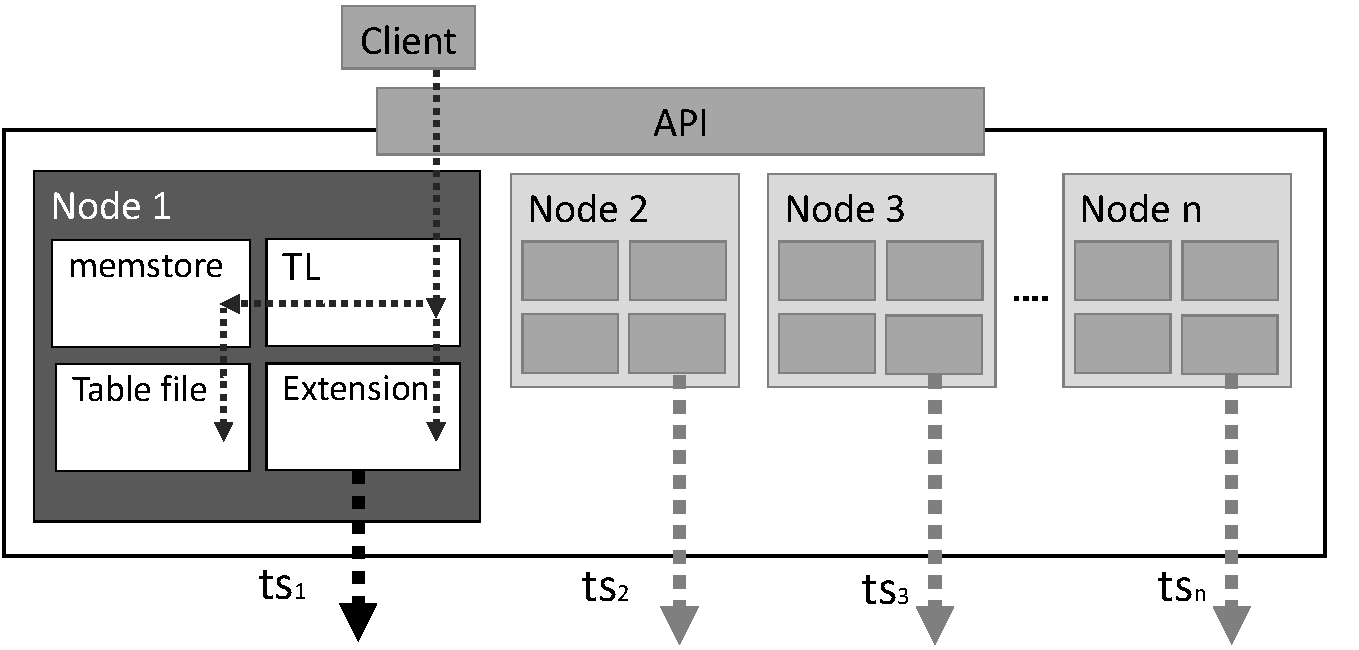
\includegraphics[width=\linewidth]{figures/KVModel} 
	\vspace{-2mm}	
	\caption{KV-model} 
	 \vspace{-2mm}
	\label{fig:kv_model} 
\end{figure} 

\subsection{API and Read/Write Path}

The \KVS\ API supports three client-side \textit{operations}:
\textit{put}, which inserts a record, \textit{get}, which retrieves a
record, and \textit{delete}, which removes a record\footnote{Sometimes
  there are additional methods, e.g., a range scan or passing a
  selection predicate to the store. However, none of them extends
  beyond repeated single row access; none of them offers expressive
  semantics.}.

In the read/write path, when reading or updating a table record,
requests pass through as few nodes as possible to reduce access
latency.  Also, a \KVS\ aims to distribute client requests among all
system nodes to spread load. For example, \HB\ routes client requests
from a root node down to the serving node in a hierarchical
manner. \CAS, on the other hand, lets clients connect to an arbitrary
node which forwards the request to the serving node.

Every node maintains a \textit{transaction log} (\TL), referred to a
write-ahead log in \HB\ and commit log in \CAS.  When a client
operation arrives, it is first written into the \TL\ of the node
(cf. Figure~\ref{fig:kv_model}). From then on, the operation is
durably persisted.  Subsequently, the operation is inserted into a
\textit{memstore}.  Memstores are volatile; upon node crash, they are
recovered from the \TL, which contains the operation sequence a node
saw over time.  During recovery, this sequence is replayed from the
log. Once a memstore exceeds a set capacity, it is flushed to disk.
Continuous flushes produce a set of table files, which are
periodically merged by a compaction process. After a flush, the
corresponding entries in the \TL\ are purged.

%\subsection{KV-store Data Model}
%
%The data model of a \KVS\ differs from that of a relational DBMS.  We
%propose a model that is representative for today's \KVSs. The model
%serves throughout the paper to help specify views and view update
%programs. Typically, \KVSs\ do not required fixed data schemas, but
%rather accommodate dynamic schema changes.
%
%Thus, we formalize the data model of a \KVS\ as a map of key-value
%pairs $\{\langle k_1, v_1\rangle,..,\langle k_n,v_n\rangle\}$
%described by a function $f:K \rightarrow V$. Systems like \BT,
%\HB\ and \CAS\ established data models that are multi-dimensional maps
%storing a row together with a variable number of columns per row. For
%example, the 2-dimensional case creates a structure
%$\{\langle(k_1,c_1),v_{1,1}\rangle,\langle (k_n,c_n)
%,v_{n,n}\rangle\}$ with a composite key $(k_n,c_n)$ that maps to a
%value $v_{n,n}$ described by $f:(K,C)\rightarrow V$. In the
%3-dimensional case, another parameter, a timestamp, for example, is
%added to the key, which may serve versioning purposes. For this paper,
%the 2-dimensional model suffices.\footnote{Our approach also works
%  with the 1-dimensional case, which is representative for simple
%  key-blob stores.  We use the 2-dimensional case, here, as it is more
%  expressive.}
%
%We denote a table by $A = (K, F)$, where $K$ represents the row key
%and $F$ a \textit{column family}. Column families are defined when a
%table is created. They are used in practice to group and access sets
%of column-value pairs. In terms of our data model, column families are
%optional. They can be dynamically assigned as the row is created. Let
%a base table row $a \in A$ be defined as $a=(k,\{\langle
%c_1,v_1\rangle..\langle c_n,v_n\rangle\})$. In this notation, the row
%key $k$ comes first, followed by a set of column-value pairs
%$\{\langle c_1,v_1\rangle..\langle c_n,v_n\rangle\}$ belonging to the
%column family. This notation more closely resembles a database row and
%is used throughout the remainder of this paper. When using multiple
%column families, we define a table as $A = (K, F_1,...F_n)$. Then, the
%assignment of a column-value set to a column family $F_x$ is denoted
%by $\{..\}_x$. The corresponding row would be defined as $a=(k,
%\{\langle c_1,v_1\rangle..\langle c_i, v_i\rangle\}_1..., \{\langle
%c_{i+1},v_{i+1}\rangle.. \langle c_n,v_n\rangle\}_n)$.


\subsection{Extension points}

We designed \VMS\ to react to \KVS\ events and to not interfere with
store-internal read/write paths for data processing. In this spirit,
we determined a number of common ``extension points,'' all considered
\KVSs\ exhibit.  We characterize extension points by events, which the
\VMS\ reacts to in maintaining views.  There are two different kinds
of events that \VMS\ needs to react to: \textit{administrative events}
and \textit{data events}.

Administrative events occur during a state change in the
\KVS\ infrastructure, e.g., a new node is added (and starts processing
client operations).  \KVSs\ provide different ways to react to
administrative events. For example, \HB\ lets developers use various
kinds of \textit{coprocessors}, which refer to application-developer
provided code pieces that can be deployed and run on system nodes
before or after certain events. We leverage this mechanisms to notify
\VMS, as soon as certain events of interest occur (e.g., the addition
of a node.)  \VMS\ reacts accordingly and allocates resources to
maintain view tables that depend on the newly added node.

%\begin{table}[h]
%\rowcolors{2}{gray!10}{gray!30}
%\setlength{\belowrulesep}{0pt}
%\setlength{\aboverulesep}{0pt}
%\setlength\extrarowheight{2pt}
%\begin{center}
%\begin{tabular}{l l l}
%\toprule
%Component & Event & Method \\
%\midrule
%Node       & added         & \textit{onNodeAdded()}  \\
%           & removed       & \textit{onNodeRemoved()}    \\
%Key-range  & opened        & \textit{onKeyRangeOpened()}\\
%           & closed        & \textit{onKeyRangeClosed()} \\
%           & split         & \textit{onKeyRangeSplit()} \\
%           & moved         & \textit{onKeyRangeMoved()} \\
%%Transaction log & replay & \textit{onTLReplay()}\\
%% & purge & \textit{onTLpurge()} \\ 
%\bottomrule 
%\end{tabular}
%\caption{Administrative events}
%\label{tab:kvs_a_events}
%\end{center}
%\end{table}


Data events occur, when a client updates a base table (e.g., put,
delete). Consequently, base table derived view tables become stale and
\VMS\ needs to update them. Generally speaking, there are three
methods to stream updates on base data from the \KVS\ to \VMS: (1)
Access the store's API, (2) intercept operations (e.g., via
coprocessors), (3) read the \TL.

Method~1 may lead to inconsistent view states, as base data 
change, before a prior update can be retrieved; none of the popular
\KVSs\ offers snapshot isolation. Also, this method would incur a lot
of overhead (e.g., an update would trigger a read and one or more
write to update derived views.)  Method~2 looks promising, especially,
with regard to freshness of the view (coprocessor execution is
synchronous in the update path), but it is only suitable if the number
of maintained views is small, otherwise \KVS\ operations would be
needlessly delayed, counter-acting the asynchronous operation behind
many design decisions. Thus, Method~3 is the preferred choice.

Method~3 has several benefits: (i) Reading \TL\ is asynchronous and
decouples processing. It neither interferes with update processing,
i.e., no latency is added into the update path, nor imposes additional
load.\footnote{Our experiments confirmed that the penalty of reading
  from the file system are far smaller than intercepting events.} (ii)
Moreover, maintaining numerous views at once means that every base
table operation generates multiple view updates. Using \TL, we
decouple view update from client operation. (iii) Operations in
\TL\ are durably persisted and can be recovered by \VMS. (iv) The 
\TL\ contains operations, not table rows, which is fine for 
incremental maintenance.



%The \KVS\ writes operations, that is client requests, to the \TL, but
%not entire table rows.  In contrast, a table row stores the row state,
%which may result from multiple client requests.  Then, an operation $t
%\in T$ can easily be defined over table row $a \in A$, with $T =
%type(A)$ and $type \in \{put, delete\}$. A put operation in the
%\TL\ is denoted as $t=put (k, \{\langle c_1,v_1\rangle..\langle
%c_n,v_n\rangle\})$. A put inserts or updates the column values at the
%specified row key. A delete operation $t \in T$ is defined as
%$t=delete (k, \{\langle c_1,\emptyset\rangle..\langle
%c_n,\emptyset\rangle\})$.  Note that we are leaving the values empty;
%the client just specifies the row key and columns that are to be
%deleted. A stream that is the output of one node's \TL\ is denoted as
%a sequence of operations $ts \in TS=(T_1,..,T_n)$. Finally, we can
%define the complete output of the \KVS\ as a set of operation streams
%as $ts_1,..ts_n \in TS$.

%
% aj - above - should we outline the difficulties imposed by not
%              having the values avail. for a delete?
%              Not mission critical.
